\documentclass[20pt]{extreport}
\usepackage[bookmarks=true,pdfstartview=FitH]{hyperref}
\usepackage{graphicx}
\usepackage{amsmath}
\usepackage{setspace}
\usepackage{ifthen}
\usepackage[letterpaper, landscape, margin=0.875in, bottom=0.5in, total={9.5in,7in}]{geometry}
\addtolength{\voffset}{-40pt}
\usepackage[document]{ragged2e}
\usepackage{fancyhdr}
\pagestyle{fancy}
\renewcommand{\headrulewidth}{0pt}
\usepackage[usenames,dvipsnames]{color}
\usepackage{color}
\lfoot{\small \color{Gray} Schlumberger Private}   %footer
\usepackage{url}
\rfoot{\includegraphics[width=10in]{"PYVARLOGO"}}
\cfoot{\break\thepage}
\linespread{1.2}
\usepackage{booktabs}
\usepackage{eso-pic}
\usepackage{transparent}
\newcommand{\tabitem}{~~\llap{\textbullet}~~}
\newcommand{\subtabitem}{~~\llap{\textendash}~~}
\newcommand{\itab}{~~\llap{}~~}
\newcommand{\tab}[1]{\hspace{.2\textwidth}\rlap{#1}}


\begin{document}     %page 1
\pdfbookmark[0]{FEA Report}{tg}
\vspace*{2pt}
\begin{center}
\begin{tabular}{l}
\LARGE\color{Blue} {Finite Element Analysis of Bit Body}\\\\
\LARGE\color{Blue}\textbf {PYVARBITNAME}\\\\
\large PYVARECO  \\
\large Analyst: PYVARUSER  \\
\large GeMS \#: PYVARGEMSNUM  Rev PYVARGEMSREV \\
\large {Date: {\today}}\\
\end{tabular}
\end{center}
\AddToShipoutPicture*{
\put(0,0){
\parbox[b][\paperheight]{\paperwidth}{%
\vfill
\centering
{\includegraphics[width=6.5in]{"PYVARDES"}}
\vfill
}
}
}


\newpage   %Page 2
\pdfbookmark[0]{BitBody -FaceView}{FaceView}
\flushleft
{\LARGE\color{Blue}\textbf {BitBody -FaceView}}
\noindent {\color{OliveGreen} \rule{\linewidth}{0.125in}}
\begin{center}
    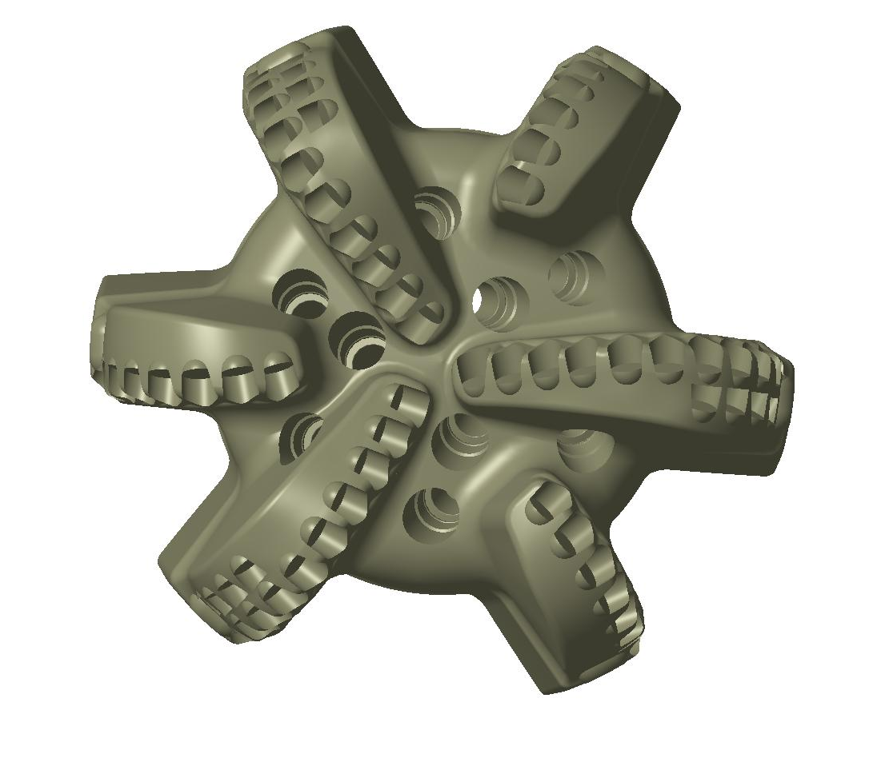
\includegraphics[width=9in,height=6in,keepaspectratio]{BitBodyFaceView}
\end{center}


\newpage   %Page 3
\pdfbookmark[0]{BitBody -RightView}{RightView}
\flushleft
{\LARGE\color{Blue}\textbf {BitBody -RightView}}
\noindent {\color{OliveGreen} \rule{\linewidth}{0.125in}}
\begin{center}
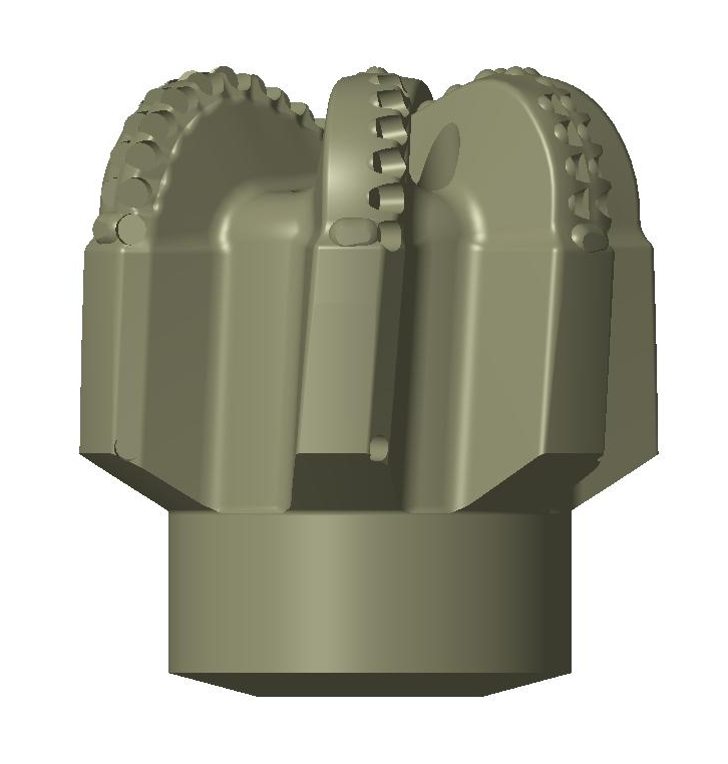
\includegraphics[width=9in,height=6in,keepaspectratio]{BitBodyRightView}
\end{center}


\newpage   %Page 4
\pdfbookmark[0]{BHA}{BHA}
\flushleft
{\LARGE\color{Blue}\textbf {BHA}}
\noindent {\color{OliveGreen} \rule{\linewidth}{0.125in}}
\begin{center}
\includegraphics[width=8in,height=6in]{PYVARIMGBHA}
\end{center}


\newpage   %Page 5
\pdfbookmark[0]{Well}{Well}
\flushleft
{\LARGE\color{Blue}\textbf {Well}}
\noindent {\color{OliveGreen} \rule{\linewidth}{0.125in}}
\begin{center}
\includegraphics[width=8in,height=6in]{PYVARIMGWELL}
\end{center}


\newpage   %Page 6
\pdfbookmark[0]{Formation And Running Parameters}{FRP}
\flushleft
{\LARGE\color{Blue}\textbf {Formation And Running Parameters}}
\noindent {\color{OliveGreen} \rule{\linewidth}{0.125in}}
\vspace{0.5in}
\large\color{Blue}\textbf {Formation - PYVARFORMATION}
\newline
\tab \large {WOB - PYVARWOB - klbf}
\newline
\tab \large {Total RPM - PYVARRPM}


\newpage   %Page 7
\pdfbookmark[0]{Cutter Force Distribution}{CF}
\flushleft
{\LARGE\color{Blue}\textbf {Cutter Force Distribution}}
\noindent {\color{OliveGreen} \rule{\linewidth}{0.125in}}
\begin{center}
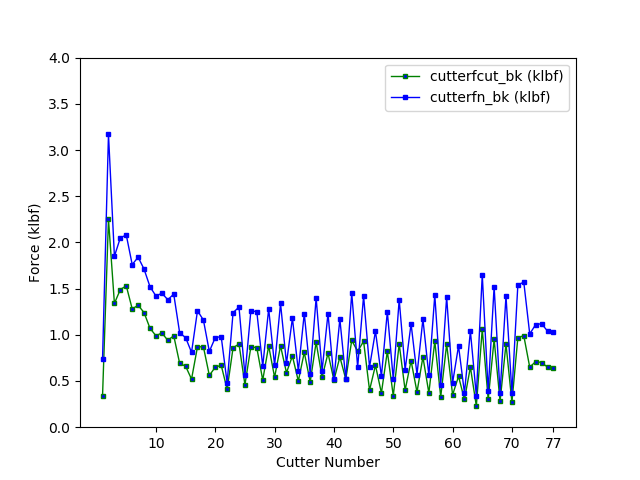
\includegraphics[width=9in,height=6in,keepaspectratio]{CutterForce}
\end{center}


\newpage   %Page 8
\pdfbookmark[0]{WOB}{WOB}
\flushleft
{\LARGE\color{Blue}\textbf {WOB}}
\noindent {\color{OliveGreen} \rule{\linewidth}{0.125in}}
\begin{center}
\includegraphics[width=6in]{PYVARIMGWOB}
\includegraphics[width=3in]{PYVARIMGWOK}
\end{center}


\newpage   %Page 9
\pdfbookmark[0]{Bit Stability}{Bit Stab}
\flushleft
{\LARGE\color{Blue}\textbf {Bit Stability}}
\noindent {\color{OliveGreen} \rule{\linewidth}{0.125in}}
\begin{center}
\includegraphics[width=6in]{PYVARAX}
\includegraphics[width=6in]{PYVARAY}
\end{center}


\newpage   %Page 10
\pdfbookmark[0]{Mesh}{Msh}
\flushleft
{\LARGE\color{Blue}\textbf {Mesh}}
\noindent {\color{OliveGreen} \rule{\linewidth}{0.125in}}
\begin{center}
\includegraphics[height=5in]{PYVARMESHIMG}
\end{center}


\newpage   %Page 11
\pdfbookmark[0]{Loading And Boundary Conditions}{BC}
\flushleft
{\LARGE\color{Blue}\textbf {Loading And Boundary Conditions}}
\noindent {\color{OliveGreen} \rule{\linewidth}{0.125in}}
\begin{center}
\includegraphics[height=5in]{PYVARCSTRIMG}
\end{center}

\newpage   %Page 12
\pdfbookmark[0]{PYVARADDSTRESS Stress Plot}{ADS}
\flushleft
{\LARGE\color{Blue}\textbf {PYVARADDSTRESS Stress Plot}}
\noindent {\color{OliveGreen} \rule{\linewidth}{0.125in}}
\vspace{0.1in}
\begin{center}
\includegraphics[height=5in]{PYVARADDIMG}
\end{center}

\newpage   %Page 13
\pdfbookmark[0]{PYVARSTRESSTYPE Stress Plot}{S}
\flushleft
{\LARGE\color{Blue}\textbf {PYVARSTRESSTYPE Stress Plot}}
\noindent {\color{OliveGreen} \rule{\linewidth}{0.125in}}
\vspace{0.1in}
\begin{center}
\includegraphics[height=5in]{PYVARMAXPIMG}
\end{center}

\newpage   %Page 14
\pdfbookmark[0]{PYVARSTRESSTYPE Face Stress Plot}{FS}
\flushleft
{\LARGE\color{Blue}\textbf {PYVARSTRESSTYPE  Face Stress Plot}}
\noindent {\color{OliveGreen} \rule{\linewidth}{0.125in}}
\vspace{0.1in}
\begin{center}
\includegraphics[height=5in]{PYVARFACESTRESS}
\end{center}


\newpage   %Page 15
\pdfbookmark[0]{Conclusions}{cnl}
\flushleft
{\LARGE\color{Blue}\textbf {Conclusions}}
\noindent {\color{OliveGreen} \rule{\linewidth}{0.125in}}
\justify
\vspace{10pt}

\large Design Bit : PYVARBITNAME\\
\large Bit BOM : PYVARBITBOM\\
\vspace{10pt}

\begin{flushleft}
 \begin{tabular}{||c|c|c|c|c||} 
 \hline
 \small Material & \small Elastic Modulus & \small Poisson's Ratio & \small Material Strength & \small Limit Strength \\ [0.5ex]
 \small  & \small (ksi) & \small  & \small (ksi)  & \small (ksi)\\ [0.5ex]  
 \hline\hline
 \newline
PYVARMATPROP
 \hline
 \end{tabular}
 \end{flushleft}

 \vspace{10pt}
 \begin{flushleft}
 \begin{tabular}{||c|c||} 
 \hline
 \small PYVARSTRESSTYPE stress in the Model & \small Result \\ [0.5ex]
 \small  (ksi) & \small $<$PASS/FAIL$>$ \\ [0.5ex]  
 \hline\hline
 \newline
\small  PYVARMAXSTRESS & \textbf{PYVARCOMPARE} \\ [0.5ex] 
 \hline
 \end{tabular}
 \end{flushleft}
\end{document}
